\documentclass[a4paper,fleqn,12pt]{article}
%\usepackage[T1]{fontenc}
\usepackage[brazilian]{babel}
%\usepackage[utf8]{inputenc}
\usepackage[left=2.5cm,right=2.5cm,top=3cm,bottom=2.5cm]{geometry}
\usepackage{mathtools}
%\usepackage{amsthm}
%\usepackage{amsmath}
%\usepackage{nccmath}
%\usepackage{amssymb}
\usepackage{amsfonts}
\usepackage{physics}
%\usepackage{dsfont}
%\usepackage{mathrsfs}

\usepackage{titling}
\usepackage{indentfirst}

\usepackage{bm}
\usepackage[dvipsnames]{xcolor}
\usepackage{cancel}

\usepackage{xurl}
\usepackage[colorlinks=true]{hyperref}

% code
\definecolor{bg}{rgb}{0.90,0.90,0.90}
\usepackage{minted}


%\usepackage{float}
%\usepackage{graphicx}
%\usepackage{tikz}
%\usepackage{caption}
%\usepackage{subcaption}

%%%%%%%%%%%%%%%%%%%%%%%%%%%%%%%%%%%%%%%%%%%%%%%%%%%

\newcommand{\eps}{\epsilon}
\newcommand{\vphi}{\varphi}
\newcommand{\cte}{\text{cte}}

\newcommand{\N}{\mathbb{N}}
\newcommand{\Z}{\mathbb{Z}}
\newcommand{\Q}{\mathbb{Q}}
\newcommand{\R}{\mathbb{R}}
%\newcommand{\C}{\mathbb{C}}
\renewcommand{\H}{\hat{H}}
\newcommand{\intR}{\int_{-\infty}^{\infty}}

\newcommand{\0}{\vb{0}}
\newcommand{\1}{\mathds{1}}
\newcommand{\E}{\vb{E}}
\newcommand{\B}{\vb{B}}
\renewcommand{\v}{\vb{v}}
\renewcommand{\r}{\vb{r}}
\renewcommand{\k}{\vb{k}}
\newcommand{\p}{\vb{p}}
\newcommand{\q}{\vb{q}}
\newcommand{\F}{\vb{F}}

\renewcommand{\a}{\hat{a}}
\renewcommand{\b}{\hat{b}}
\renewcommand{\c}{\hat{c}}
\newcommand{\nn}{\hat{n}}

\newcommand{\gf}[2]{\ev{\ev{#1 : #2}}}
\newcommand{\zub}[2]{\ev{\comm{#1}{#2}_\mp}}

\newcommand{\s}[1]{\mathcal{#1}}
%\newcommand{\prodint}[2]{\left\langle #1 , #2 \right\rangle}
\newcommand{\cc}[1]{\overline{#1}}
\newcommand{\Eval}[3]{\eval{\left( #1 \right)}_{#2}^{#3}}

\newcommand{\unit}[1]{\; \mathrm{#1}}

\newcommand{\n}{\medskip}
\newcommand{\e}{\quad \mathrm{e} \quad}
\newcommand{\ou}{\quad \mathrm{ou} \quad}
\newcommand{\virg}{\, , \;}
\newcommand{\ptodo}{\forall \,}
\renewcommand{\implies}{\; \Rightarrow \;}
%\newcommand{\eqname}[1]{\tag*{#1}} % Tag equation with name

% math %
\renewcommand{\erf}[1]{\text{erf}\left(#1\right)}
\newcommand{\floor}[1]{\left\lfloor #1 \right\rfloor}
\newcommand{\ceil}[1]{\left\lceil #1 \right\rceil}

\setlength{\droptitle}{-6em}


\title{\Huge{\textbf{P2 - Statistical Learning}}}
\author{Mateus Marques}

\begin{document}

\maketitle

\section{Neural Networks}

Para complementar os slides horríveis do professor, ler as páginas 403-424 do livro \textit{Statistical Learning} (veja o \texttt{README.md}).

\subsection{Perceptron}

Perceptron são funções simples assim:
$$
Y = f\qty(w_0 + \sum_{i=1}^{n} w_i X_i),
$$
onde $f(X) = 1$ se $X \geq 0$, e $-1$ caso contrário.

Só que os perceptrons só conseguem resolver problemas linearmente separáveis (tipo SVM).
\begin{figure}[H]
\centering
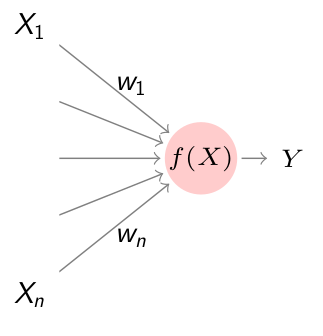
\includegraphics[width=0.3\textwidth]{fig/perceptron.png}
\caption{Perceptron.}
\label{fig:perceptron}
\end{figure}

\subsection{Multi-Layer Perceptron (MLP)}

Com novas camadas temos mais liberdade:
$$
Y =  \beta_0 + \sum_{k=1}^{K} \beta_k \, g\qty(w_{k0} + \sum_{j=1}^{p} w_{kj} X_k),
$$
onde $p$ é o número de variáveis na camada de input e $K$ o número de variáveis na camada oculta.
\begin{figure}[H]
\centering
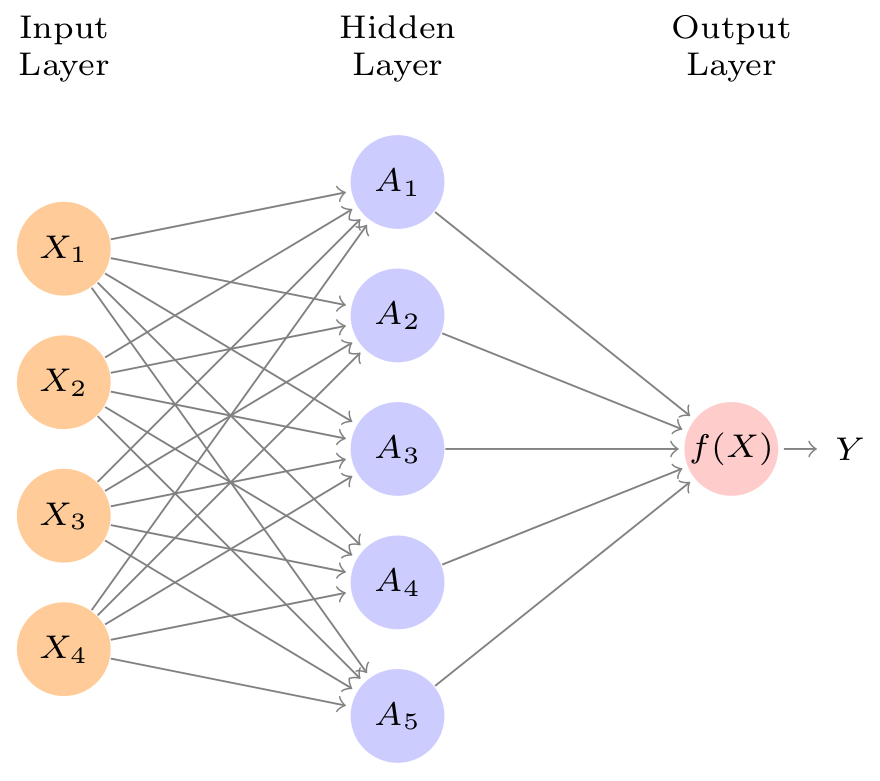
\includegraphics[width=0.4\textwidth]{fig/mlp.png}
\caption{Multi-Layer Perceptron (MLP).}
\label{fig:mlp}
\end{figure}

Com apenas uma camada oculta, a função de ativação $g(\cdot)$ deve ser não-linear, do contrário teremos uma estrutura linear. Geralmente escolhemos $g(z)$ assim:
\begin{figure}[H]
\centering
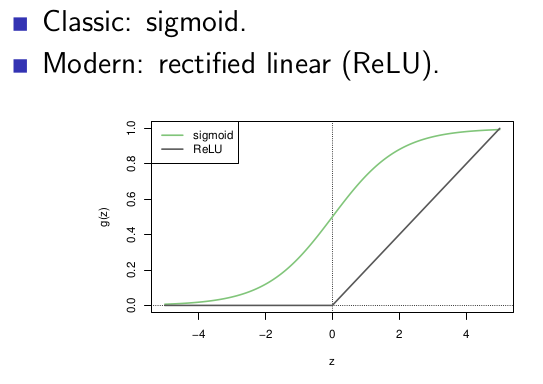
\includegraphics[width=0.4\textwidth]{fig/activation_function.png}
\caption{Função de ativação.}
\label{fig:units_activation_functions}
\end{figure}

Existe o chamado \textbf{Universal Approximation Result (1989)}: um Multi-Layer Perceptron (MLP) com uma única camada oculta consegue aproximar qualquer função contínua arbitrariamente bem.
\begin{figure}[H]
\centering
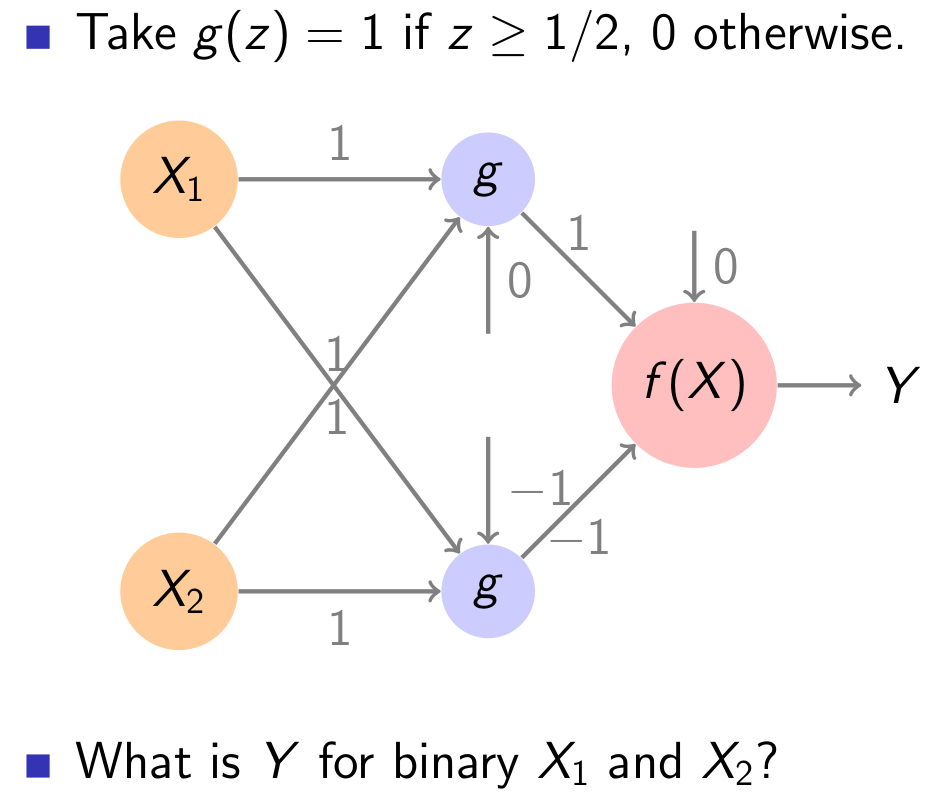
\includegraphics[width=0.5\textwidth]{fig/example_mlp.png}
\caption{Exemplo de Multi-Layer Perceptron (MLP).}
\label{fig:example_mlp}
\end{figure}

No exemplo acima, os pesos são:
$$
\begin{cases}
\; \beta_0 = 0, \beta_1 = 1, \beta_2 = -1; \\
\; w_{10} = 0 , w_{11} = 1, w_{12} = 1; \\
\; w_{20} = -1, w_{21} = 1, w_{22} = 1.
\end{cases}
$$
Isso nos dá que
$$
Y = g\qty(X_1 + X_2) - g\qty(X_1 + X_2 - 1),
$$
onde $g(z) = 1$ se $z \geq 1/2$ e $g(z) = 0$ caso contrário.

Com muitos outputs, a esquematização é desse jeito:
\begin{figure}[H]
\centering
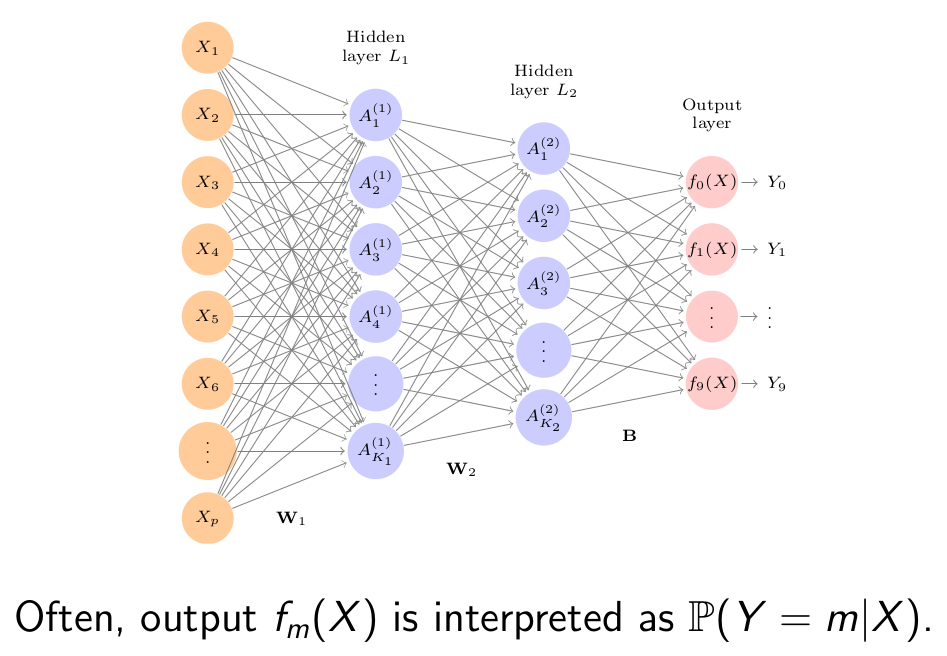
\includegraphics[width=0.6\textwidth]{fig/many_outputs.png}
\caption{Esquematização de muitos outputs.}
\label{fig:many_outputs}
\end{figure}



\end{document}
